% Chapter 1

\chapter{Introducción general} % Main chapter title

\label{Chapter1} % For referencing the chapter elsewhere, use \ref{Chapter1} 
\label{IntroGeneral}

%----------------------------------------------------------------------------------------

% Define some commands to keep the formatting separated from the content 
\newcommand{\keyword}[1]{\textbf{#1}}
\newcommand{\tabhead}[1]{\textbf{#1}}
\newcommand{\code}[1]{\texttt{#1}}
\newcommand{\file}[1]{\texttt{\bfseries#1}}
\newcommand{\option}[1]{\texttt{\itshape#1}}
\newcommand{\grados}{$^{\circ}$}

%----------------------------------------------------------------------------------------

%\section{Introducción}

%----------------------------------------------------------------------------------------
\section{Introducción a la domótica}

La domótica es la aplicación de la tecnología a la automatización del hogar y de edificios que utiliza para controlar y gestionar diferentes sistemas y dispositivos en el hogar o edificio de forma automatizada, con el fin de aportar seguridad, bienestar y confort. Estos sistemas pueden incluir iluminación, calefacción, aire acondicionado, sistemas de seguridad y cámaras de vigilancia, sistemas de entretenimiento y otros dispositivos domésticos. \citep{1}

Este sector como muchos otros que utilizan tecnología ha estado creciendo, al punto que algunas de las viviendas modernas son concebidas como hogares inteligentes desde su edificación, llegando a tener edificios completos con este tipo de soluciones instaladas.

\subsection{Aplicaciones}

Los servicios que ofrece la domótica se pueden agrupar según cinco aspectos o ámbitos principales \citep{2}:

\begin{itemize}
	\item Programación y ahorro energético. El ahorro energético no es algo tangible, sino legible con un concepto al que se puede llegar de muchas maneras. En muchos casos no es necesario sustituir los aparatos o sistemas del hogar por otros que consuman menos energía sino una gestión eficiente de los mismos.
	\item Confort. El confort conlleva todas las actuaciones que se puedan llevar a cabo que mejoren la comodidad en una vivienda. Dichas actuaciones pueden ser de carácter tanto pasivo, como activo o mixtas.
	\item Seguridad. Consiste en una red de seguridad encargada de proteger tanto los bienes patrimoniales, como la seguridad personal y la vida.
	\item Comunicaciones. Son los sistemas o infraestructuras de comunicaciones que posee el hogar.
	\item Accesibilidad. Bajo este mecanismo se incluyen las aplicaciones o instalaciones de control remoto del entorno que favorecen la autonomía personal de personas con limitaciones funcionales, o discapacidad.
\end{itemize}

El presente trabajo puede encuadrarse dentro de la programación y ahorro energético, confort y accesibilidad. En la figura \ref{fig:1} puede verse una imagen con los distintos tipos de dispositivos que pueden estar conectados a un sistema de domótica.

\begin{figure}[h]
\centering
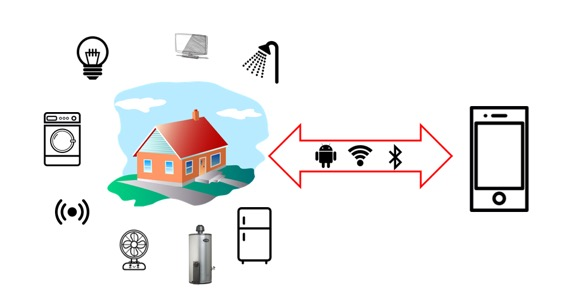
\includegraphics[scale=0.55]{Imagen 1 - Domotica.jpg}
\caption[Ejemplo de sistema de domótica]{Ejemplo de sistema de domótica. \footnotemark}
\label{fig:1}
\end{figure}
\footnotetext{Imagen tomada de: \url{https://intelligy.com/blog/2018/03/12/conoces-la-domotica/}}

\section{Motivación}

El uso de la tecnología para facilitar y mejorar la vida de las personas se está implementando en todo el mundo en diversos ámbitos creando soluciones complejas e innovadoras. Los electrodomésticos e instalaciones se fabrican con posibilidades de conexión y capacidades cada vez más amplias, abarcando funcionalidades complejas que aportan al bienestar y confort de las personas.

Este proyecto nace como la mejora y actualización de la tesis de grado de ingeniería en la cual se creó un sistema similar que carecía de conectividad a internet y utilizando tecnología que al día de hoy es obsoleta. Es por este motivo que decidí hacer un proyecto académico con esta temática, pudiendo crear un sistema integral con una página web, base de datos que almacene mediciones y utilizando hardware actualizado.
